\documentclass{cmn}
\usepackage{pgfplots}
\pgfplotsset{compat=1.18}
\usepgfplotslibrary{units}

\begin{document}
  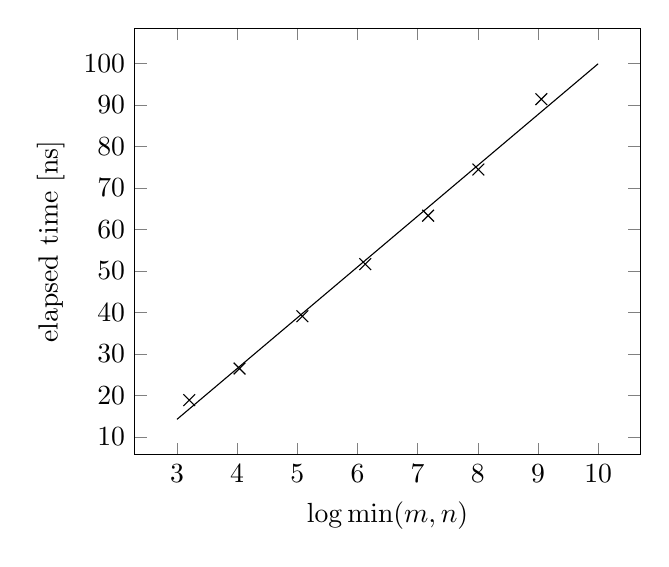
\begin{tikzpicture}
    \begin{axis}[
      width=80mm,
      height=70mm,
      xlabel={$\log \min(m, n)$},
      ylabel={elapsed time},
      use units,
      y unit=s,
      y unit prefix=n,
      xtick distance=1,
      ytick distance=10,
    ]
      \addplot[only marks,mark=x,mark size=3pt] table [x=m,y=t]{
        m                  t
        3.203304916138483  18.849
        4.0392554438064865 26.461
        5.084193644325543  39.069
        6.129131845581379  51.608
        7.174070046831225  63.312
        8.01002060783114   74.427
        9.054958809081034  91.376
      };
      \addplot [domain=3:10] { 12.24545*x - 22.53095 };
    \end{axis}
  \end{tikzpicture}
\end{document}
